% ..............................................................................
% Demo of the fau-beamer template.
%
% Copyright 2022 by Tim Roith <tim.roith@fau.de>
%
% This program can be redistributed and/or modified under the terms
% of the GNU Public License, version 2.
%
% ------------------------------------------------------------------------------
\documentclass[final]{beamer}

% ========================================================================================
% Theme: inner, outer, font and colors
% ----------------------------------------------------------------------------------------
\usepackage[institute=Tech,
			%SecondLogo = template-art/FAUWortmarkeBlau.pdf,
			%ThirdLogo = template-art/FAUWortmarkeBlau.pdf,
			%WordMark=None,
			aspectratio=169,
			fontsize=11,
			fontbaselineskip=13,
			scale=1.,
			InsertTotalFoot
		   ]{styles/beamerthemefau}
% ----------------------------------------------------------------------------------------
% Input and output encoding
\usepackage[T1]{fontenc}
\usepackage[utf8]{inputenc}
% ----------------------------------------------------------------------------------------
% Language settings
\usepackage[english]{babel}

% ========================================================================================
% Fonts
% - Helvet is loaded by styles/beamerfonts
% - We use serif for math environements
% - isomath is used for upGreek letters
% ----------------------------------------------------------------------------------------
\usepackage{isomath}
\usefonttheme[onlymath]{serif}
\usepackage{exscale}
\usepackage{anyfontsize}
\setbeamercolor{alerted text}{fg=BaseColor}
% ----------------------------------------------------------------------------------------
% custom commands for symbols
\usepackage{styles/symbols}


% ========================================================================================
% Setup for Titlepage
% ----------------------------------------------------------------------------------------
\title[fau-beamer]{DRÆM - Pitch Presentation}
\subtitle{A Discriminatively Trained Reconstruction Embedding for Surface Anomaly Detection}
\author[C. Roßbach]{
Christopher Roßbach\inst{1}}
%
\institute[FAU]{%
\inst{1} Friedrich-Alexander-Universität Erlangen-Nürnberg, Technische Fakultät
}

\date{\today}


% ================================================
% Bibliography
% ------------------------------------------------
\usepackage{csquotes}
\usepackage[style=alphabetic, %alternatively: numeric, numeric-comp, and other from biblatex
			defernumbers=true,
			useprefix=true,%
			giveninits=true,%
			hyperref=true,%
			autocite=inline,%
			maxcitenames=5,%
			maxbibnames=20,%
			uniquename=init,%
			sortcites=true,% sort citations when multiple entries are passed to one cite command
			doi=true,%
			isbn=false,%
			url=false,%
			eprint=false,%
			backend=bibtex%
		   ]{biblatex}
\addbibresource{bibliography.bib}
\setbeamertemplate{bibliography item}[text]


% ================================================
% Hyperref and setup
% ------------------------------------------------
\usepackage{hyperref}
\hypersetup{
	colorlinks = true,
	final=true, 
	plainpages=false,
	pdfstartview=FitV,
	pdftoolbar=true,
	pdfmenubar=true,
	pdfencoding=auto,
	psdextra,
	bookmarksopen=true,
	bookmarksnumbered=true,
	breaklinks=true,
	linktocpage=true,
	urlcolor=BaseColor,
	citecolor=BaseColor,
	linkcolor=BaseColor
}


% ================================================
% Additional packages
% ------------------------------------------------


% ================================================
% Various custom commands
% ------------------------------------------------
%\setbeameroption{show notes on second screen}
\begingroup\expandafter\expandafter\expandafter\endgroup
\expandafter\ifx\csname pdfsuppresswarningpagegroup\endcsname\relax
\else
  \pdfsuppresswarningpagegroup=1\relax
\fi
% Change color for cite locally
\newcommand{\colorcite}[3]{{\hypersetup{citecolor=#1}{\cite[#2]{#3}}}} 
% ------------------------------------------------
% ================================================
% The main document
% ------------------------------------------------
\begin{document}
% Title page
\begin{frame}[t,titleimage]{-}
\titlepage%
\end{frame}

% Introduction
\begin{frame}{Introduction}{Surface Anomaly Detection: Why It Matters}
    \begin{itemize}
        \item Where applied, surface anomaly detection often outperforms humans in both specificity and sensitivity while simultaneously reducing costs
        \pause
        \begin{itemize}
            \item Why is it not applied everywhere?
            \pause
            \item One problem is the availability of data, especially of rare anomalies
        \end{itemize}
        \pause
        
        \item \textbf{Paper:} ``DRÆM -- A Discriminatively Trained Reconstruction Anomaly Embedding Model for Surface Anomaly Detection''\footcite{zavrtanikDRAEMDiscriminativelyTrained2021}
        \pause
        
        \item \textbf{Why Surface Anomaly Detection Matters:}
        \begin{itemize}
            \item \textbf{Healthcare:} Detecting skin lesions, tissue abnormalities in medical imaging
            \item \textbf{Manufacturing:} Identifying defects in circuit boards, scratches on automotive parts
            \item \textbf{Infrastructure:} Finding cracks in bridges, corrosion on pipelines
            \item \textbf{Food Industry:} Spotting contamination on produce, foreign objects in packaging
            \item \textbf{Textiles, Pharmaceutical Industry, \ldots}
        \end{itemize}
    \end{itemize}
\end{frame}

\begin{frame}{Problem Statement}{Current Situation and Related Work}
    \begin{itemize}
        \item<1-> OOD-Samples are often rare and diverse
        \item<2-> Data collection for pixel accurate anomaly detection is hard
        \item<3-> Reliance on only normal data is preferred
        \begin{columns}
            \begin{column}{0.4\textwidth}
                \begin{enumerate}
                    \item<4-> Methods try to either learn compression and decompression (e.g. auto-encoders) of normal data and measure reconstruction error
                    \begin{itemize}
                        \item<5-> Hand-crafting difference functions for the first one is hard, the second suffers from less sharp anomaly borders
                    \end{itemize}
                    \item<6-> Or perform patchwise analysis of (deep) feature (e.g. CNNs) distribution deviation
                    \begin{itemize}
                        \item<7-> These often suffer from unsharp segmentation maps
                    \end{itemize}
                \end{enumerate}
            \end{column}
                \begin{column}{0.6\textwidth}
                    \uncover<4->{
                        \begin{figure}
                            \centering
                            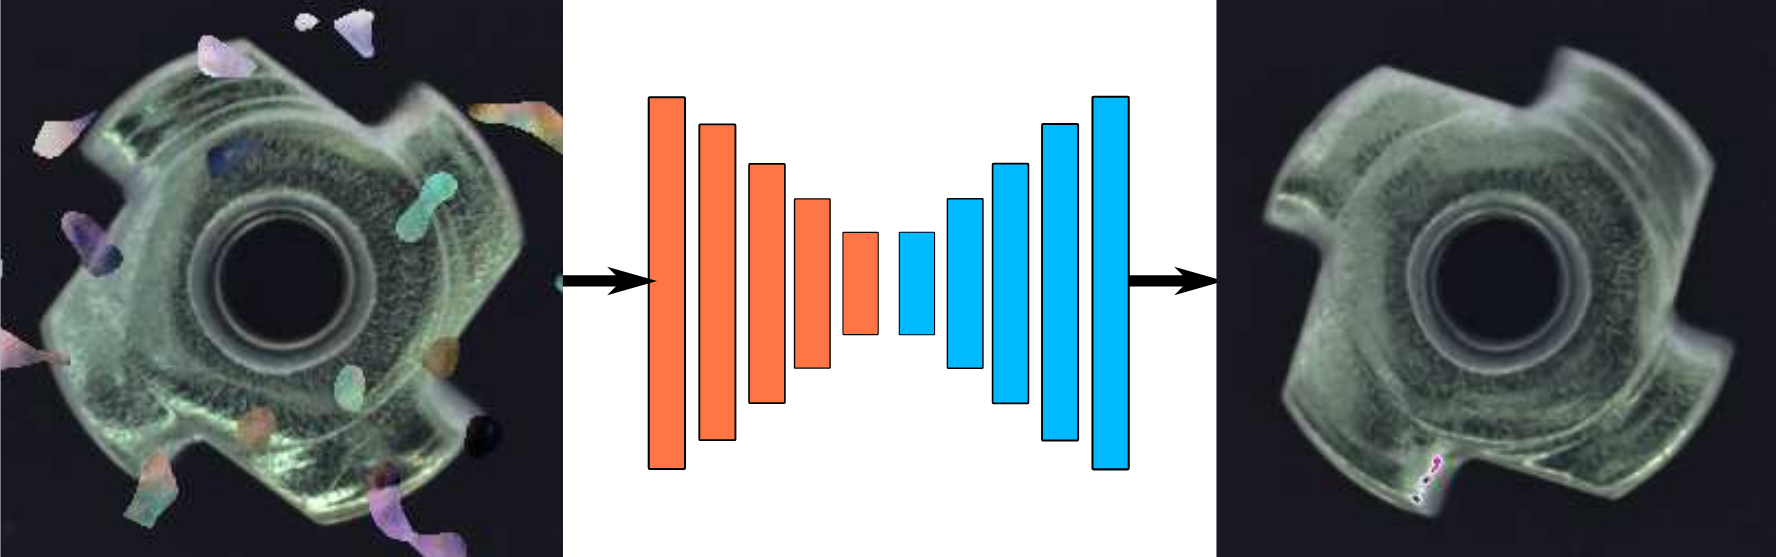
\includegraphics[width=0.8\textwidth]{pitch/auto-encoder.png}
                        \end{figure}
                    }
                    \uncover<7->{
                        \begin{figure}
                            \centering
                            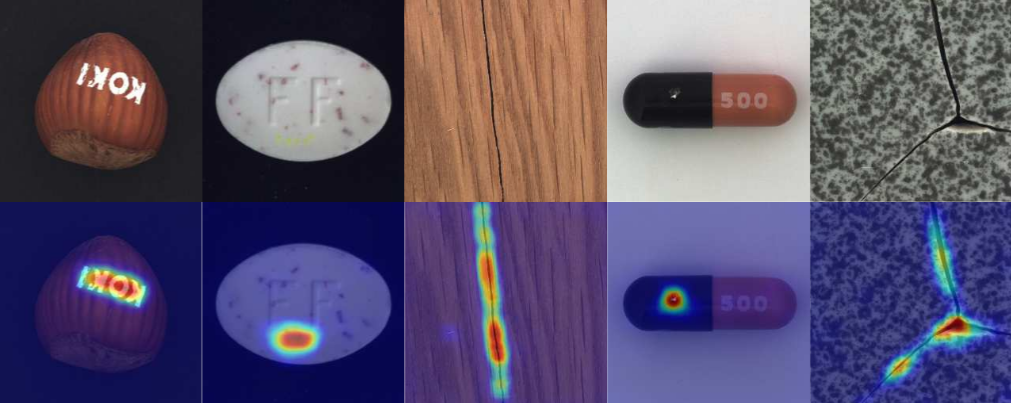
\includegraphics[width=0.8\textwidth]{pitch/unsharp-segmentation.png}
                        \end{figure}
                    }
                \end{column}
        \end{columns}
    \end{itemize}
\end{frame}

\begin{frame}{Framework Overview}{How it Works}
    \begin{center}
        \begin{tikzpicture}[scale=1.428]
            \node (img) at (0,0) {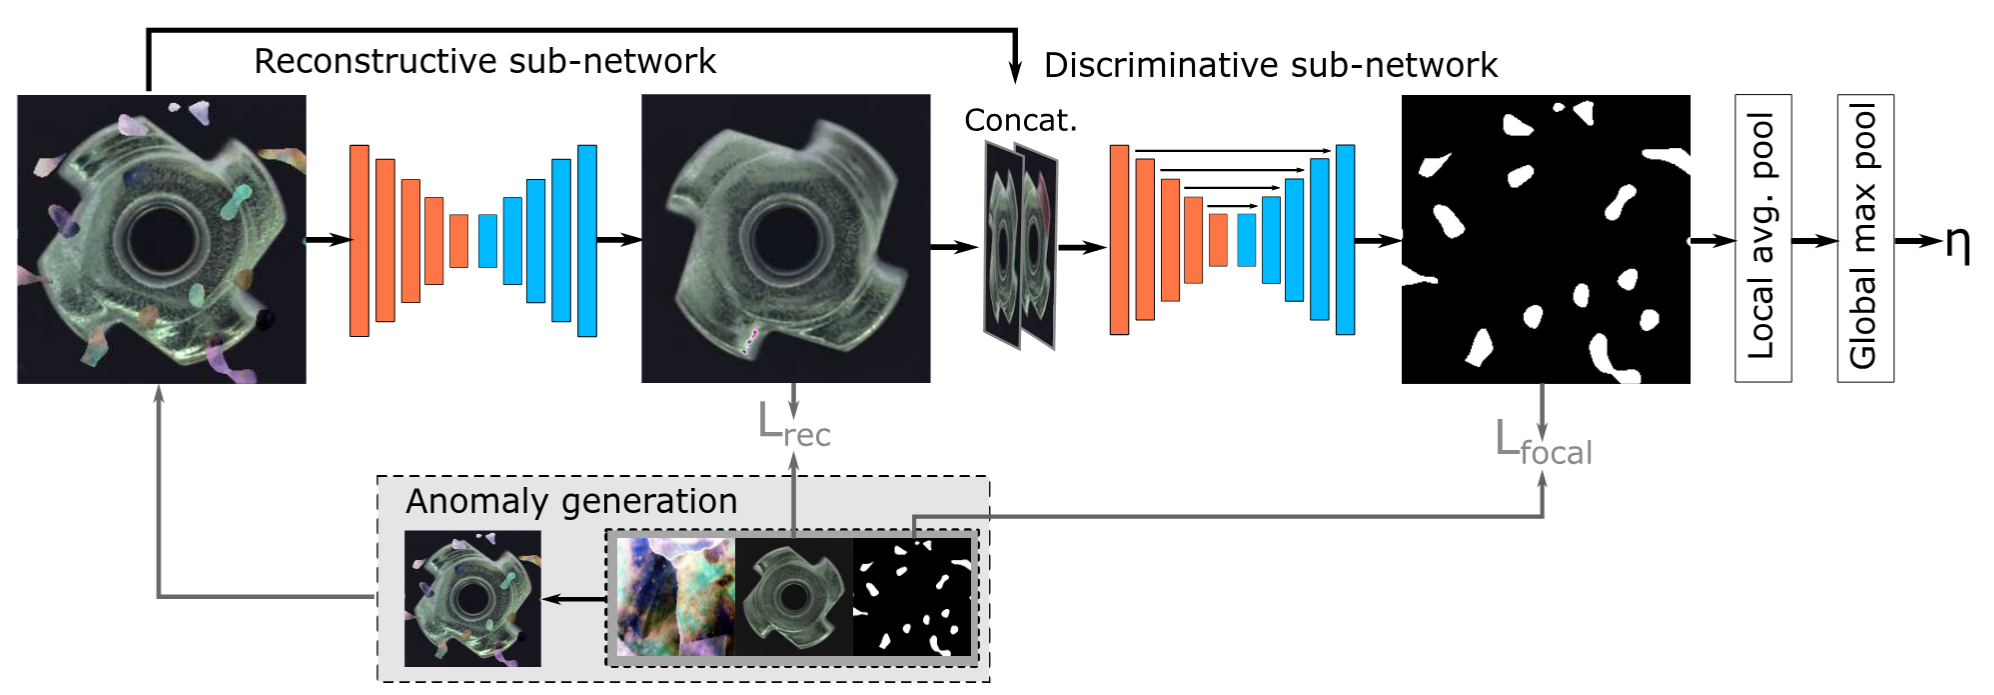
\includegraphics[width=\textwidth]{pitch/pipeline.png}};
            \uncover<-1>{
                \fill[white] (-11.5,-1.2) rectangle (8.5,4.8);
                \fill[white] (-11.5,-4.2) rectangle (-7.1,4.8);
            }
            \only<-2>{
                \fill[white] (0.0,-4.2) rectangle (11.5,4.8);
                \fill[white] (-0.5,-0.2) rectangle (11.5,4.8);
            }
            \only<-3>{
                \fill[white] (8.0,-4.2) rectangle (11.5,4.8);
            }
            \only<4>{}
        \end{tikzpicture}
    \end{center}
\end{frame}

\begin{frame}{Key Findings \& Application \& Conclusion}{The Value of DRÆM}
    \begin{columns}
        \begin{column}{0.5\textwidth}
            \begin{itemize}[<+->]
                \item Outperforms unsupervised SOTA methods
                \item Similar performance to supervised SOTA methods
                \item High quality segmentation can help downstream tasks
                \begin{itemize}
                    \item Estimate the size of impacted area
                    \item Distinguish between crack, corrosion or just paint
                \end{itemize}
                \item We don't need expensive hand-labeled data
                \item We only need just-out-of-distribution patterns for anomaly generation
            \end{itemize}
        \end{column}
        \begin{column}{0.5\textwidth}
            \uncover<3->{
                \begin{figure}
                    \centering
                    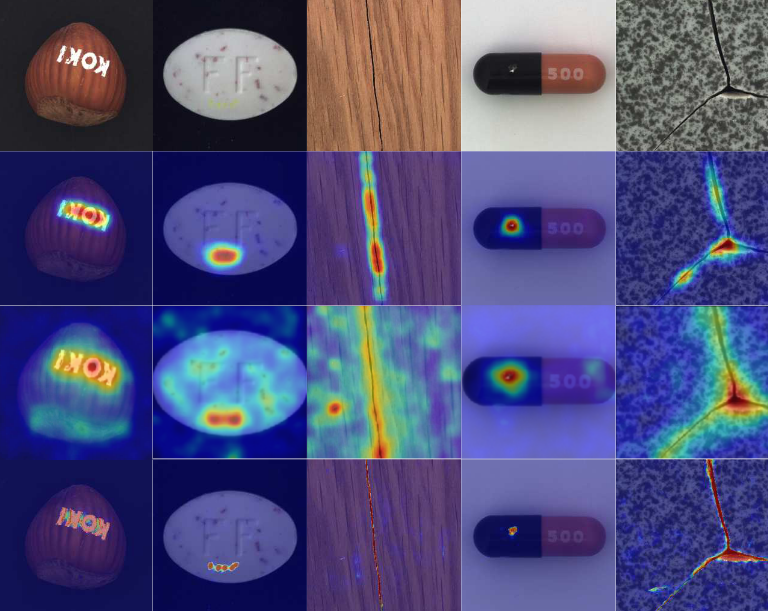
\includegraphics[width=0.9\textwidth]{pitch/sharp-segmentation.png}
                \end{figure}
            }
        \end{column}
    \end{columns}
\end{frame}

\begin{frame}{Limitation \& Extension}{Where to go from Here}
    \begin{itemize}[<+->]
        \item The method lacks performance in cases where domain knowledge is necessary to perform well
        \item For example here the whole lead of the transistor is cut off, but it only marks the position of the cut
        \begin{figure}
            \centering
            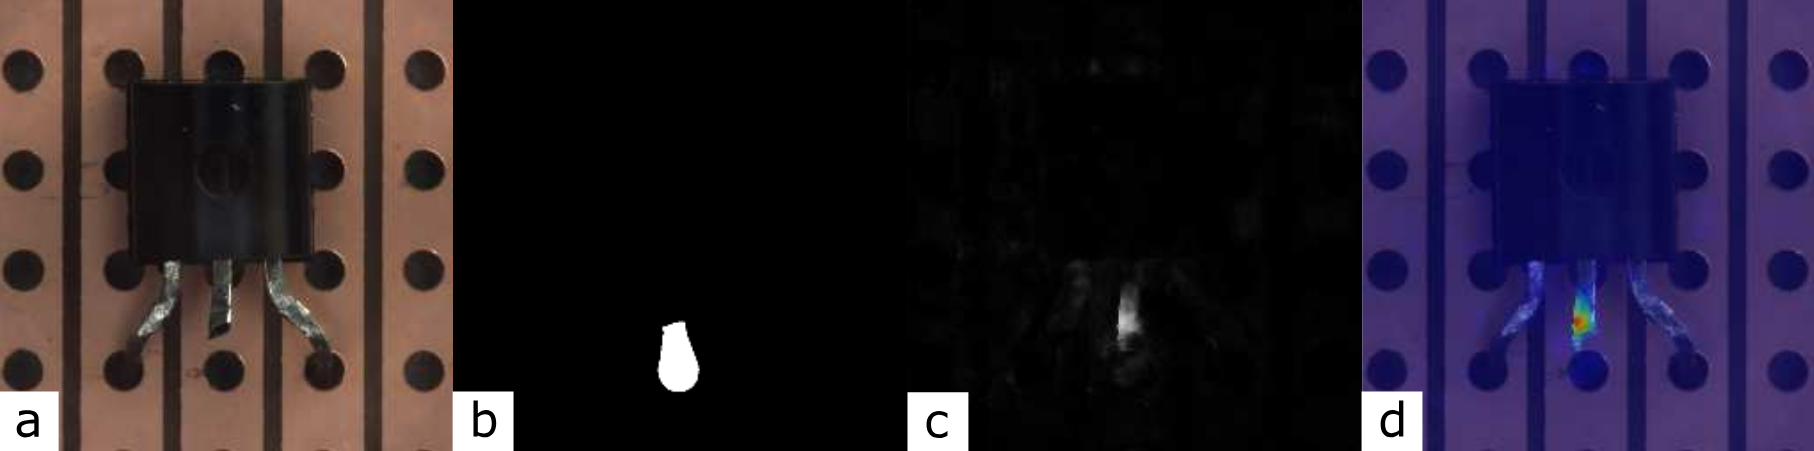
\includegraphics[width=0.5\textwidth]{pitch/transistor.png}
        \end{figure}
        \item Another example could be when certain "normalities" are underrepresented in the training data
        \begin{itemize}
            \item DRÆM may detect stains on walls as anomalies, while only structural damage should be detected
            \item In these cases finetuning the discriminative network may improve performance
        \end{itemize}
    \end{itemize}
\end{frame}

\begin{frame}[t,titleimage]{-}
    Thank you for your attention
\end{frame}

\end{document}